\chapter{Lissajous Figures and Resonance}


\section{Introduction}

In this lab, you'll view Lissajous curves in 2-D using the $X$-$Y$ mode of your scope and reproduce the same curves using parameterized equations in Scientific Python. You will also  build and measure the performance of a $RLC$ band-pass filter and determine its resonant frequency and quality (Q) factor. For this lab there are both logbook and jupyter notebook entries.

\section{Lissajous Figures}

\begin{figure}[htbp]
\begin{center}
\begin{tabular}{cc}
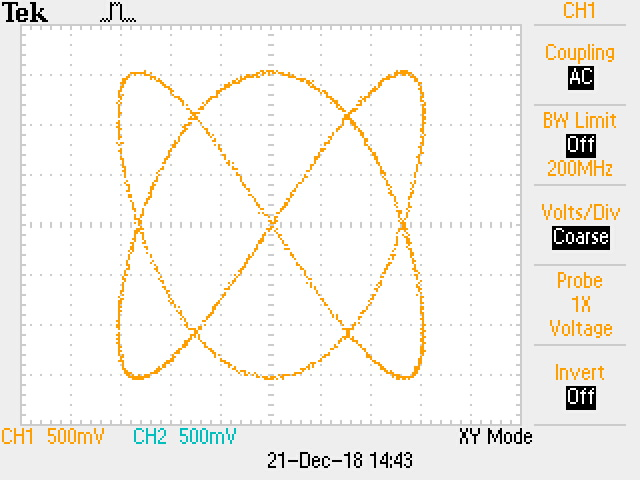
\includegraphics[width=0.45\textwidth]{figs/labs/lissajous/scope_lissajous.jpg} & 
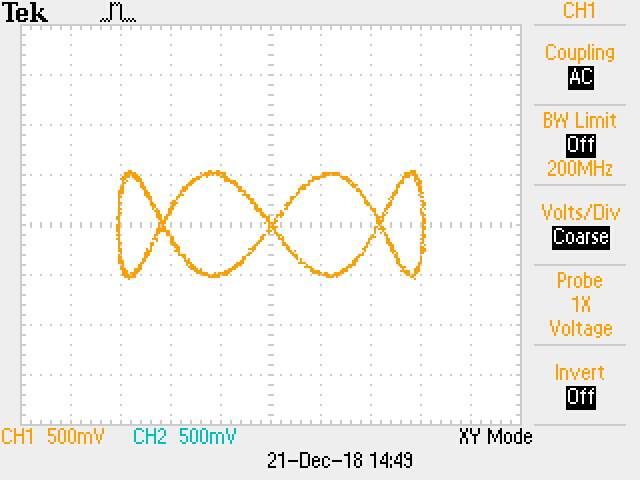
\includegraphics[width=0.45\textwidth]{figs/labs/lissajous/scope_crown.jpg} \\
(a) & (b) \\
\end{tabular}
\caption{Scope traces from Lissajous figures from settings for (a) start, and (b) crown.}
\label{fig:tracelissajous}
\end{center}
\end{figure}
Lissajous figures are the graph of system of two parameterized functions:
\begin{eqnarray*}
x &=& A_1 \sin(2 \pi f_1 t + \delta) \\
y &=& A_2 \sin(2 \pi f_2 t) 
\end{eqnarray*}
which produces a closed loop if the ratio $A_1 / A_2$ is rational.  The appearance of the figure is of a 3 dimensional knot with the viewing angle determined by the parameter $\delta$.  Two examples are shown in Fig.~\ref{fig:tracelissajous}.

To produce these figures on your scope, we'll need to use two
channels.  To begin, enable the output of both Channel 1 and Channel 2
on your function generator, and set them both to produce sine waves
with amplitude $3~\rm V$ peak-to-peak.  Adjust the frequency of
channel 1 to $2~\rm kHz$ and the channel 2 to $3~\rm kHz$.  Note that
you can switch between the Channel 1 and Channel 2 parameter menus on the function generator
with the button labeled ``Ch1/2''.

\begin{figure}[htbp]
\begin{center}
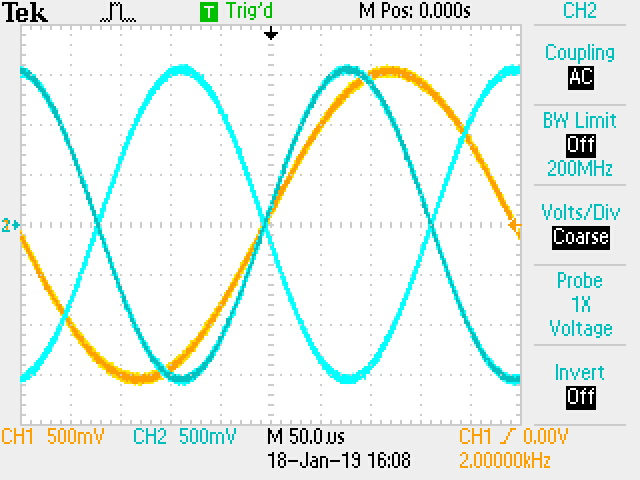
\includegraphics[width=0.45\textwidth]{figs/labs/lissajous/two_sine.jpg} 
\caption{Correctly scaled scope output.}
\label{fig:twosine}
\end{center}
\end{figure}

On your scope, switch to the Channel 2 parameter menu by pressing the
blue button labeled ``2''.  Set the coupling of Channel 2 to AC, and
probe attenuation to 1x, just as you did previously for Channel 1.
Next adjust the voltage scales of each channel to $500~\rm mV$ and set
the common time scale to something appropriate, so that you can view
both Sine waves on the scope display.  As shown in Fig.~\ref{fig:twosine},
you will see two versions of the Channel 2 output, inverted with
respect to each other, because the frequency of Channel 2 is 1.5 times
the frequency of Channel 1. You can check this but changing slightly the frequency of 
Channel 2 but return it to prescribe values to continue with the lab.

The relative phase between the two output channels of your function
generator shifts whenever you adjust the frequency of one of the
signals.  For consistent results with offline plots and the scope
traces shown here, you'll need to align the phase of the two channels
every time you adjust the frequency on the function generator:
\begin{displaymath}
\rm Inter Ch button \to AlignPhase.
\end{displaymath}

Usually, scopes are used to display the inputs as a function of time.
In this case, the voltage level is along the $y$-axis, and time is the
$x$-axis.  This mode is called YT mode.  Occasionally, however, it is
useful to display things in XY mode.  In this mode, the $x$-axis is
used for the voltage of Channel 1 and the $y$-axis is used for the
voltage of Channel 2.  Each point on the curve represents a particular
point in time.  Switch to XY mode by pressing the Display button and
then pressing the button next to the Format menu item until the mode
is XY.  You should reproduce Fig.~\ref{fig:tracelissajous}a
exactly.  If not, check that you have aligned the phase as described
above and that frequencies are set correctly as in Table.

\begin{table}
\begin{center}
\caption{Settings for various Lissajous figures.}
\label{tbl:lissajous}
\begin{tabular}{llll}
pattern & $f_1~\rm(kHz)$ & $f_2~\rm(kHz)$ & $\delta_1$ \\
start & 2 & 3 & 0 \\
fish & 2 & 3 & $135^\circ$ \\
parabola & 1 & 2 & $45^\circ$ \\
lace & 13 & 12 & 0 \\
crown & $1~\rm kHz$ & $4~\rm kHz$ & 0 \\
\end{tabular}
\end{center}
\end{table}

\begin{plot} Adjust the phase of Channel 2, under menu item StartPhase, until the
pattern collapses into a Fish pattern (or greek letter $\alpha$) at
135 degrees. Make sure that there is a date printed on the screen of your scope trace.  Save a scope trace by inserting your USB drive into the
scope and pressing the Save button (it takes few seconds to save).  \end{plot}

 \begin{plot}Then produce the parabola pattern  according to the settings in Table~\ref{tbl:lissajous}, saving a scope
trace.  Remember to align the phase each time you change the frequency.\end{plot}
\begin{plot} Produce lace pattern and save a scope trace. \end{plot}

\begin{plot} Next, produce the crown pattern, shown in Fig.~\ref{fig:tracelissajous}b.
For the right proportions, adjust the amplitude of
Channel 2 to $1~\rm V$ peak-to-peak, leaving Channel 1 at $3~\rm V$
peak-to-peak.  Notice that as you adjust the phase of Channel 1, the
crown appears to rotate.  Adjust the frequency of Channel 2 to
$4.0002~\rm kHz$.  The crown should now appear to rotate constantly at
low speed.  \end{plot}

\noindent
Include your saved scope traces of Lissajous figures in the python notebook. Provide a full label for each plot which describes all the relevant information. 

\section{Band-pass Filter}



\begin{figure}[htbp]
\begin{center}
\begin{circuitikz}[line width=1pt]
\draw (0,0) to[sinusoidal voltage source,bipoles/length=1.5cm] ++(0,3.0) 
to[R,-*,l_=$R_1$] ++(2.0,0) coordinate(X) to[short,*-*] ++(1.5,0) coordinate(Y) to[short,-o] ++(1.0,0) node[right]{B};
\draw (X) to[C,-*,l=$C_1$] ++(0,-3.0)  to[short,-*] ++(-2.0,0) node[ground,yscale=2.0]{};
\draw (Y) to[L,-*,l=$L_1$] ++(0,-3.0)  coordinate(X) to[short,-*] ++(-1.5,0);
\draw (X) to[short,-o] ++(1.0,0) node[right]{A};
\end{circuitikz}  
\caption{Circuit diagram for RLC band-pass filter.}
\label{fig:rlc_circuit}
\end{center}
\end{figure}


%\begin{figure}[htbp]
%\begin{center}
%%\begin{tabular}{c@{\hskip 0.25in}c}
%\begin{tabular}{cc}
%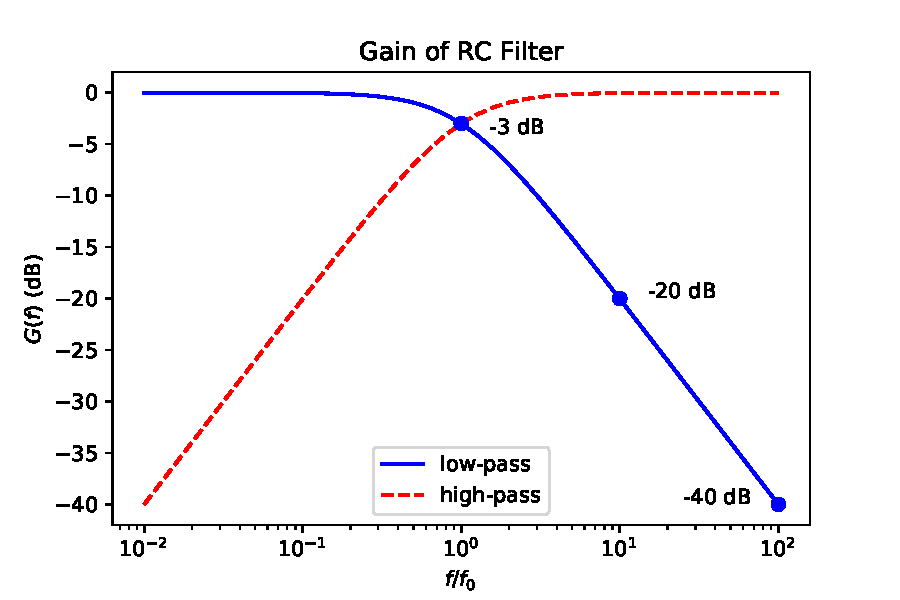
\includegraphics[height=0.22\textheight]{figs/labs/filters/rcgaindb.pdf}
%&
%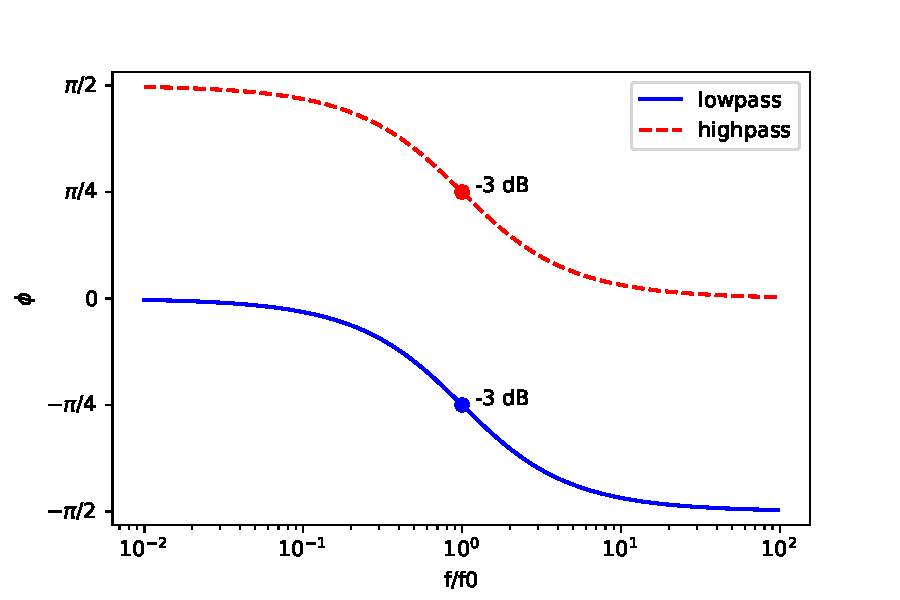
\includegraphics[height=0.22\textheight]{figs/labs/filters/rcphase.pdf} \\
%(a) & (b) \\
%\end{tabular}
%\end{center}
%\caption{\label{fig:bode} Bode plots for band-pass filter showing the (a) gain on a dB scale, and (b) phase, both as a function of the ratio of frequency $f$ to the crossover frequency $f_0$ on a log scale.}
%\end{figure}

%
%\begin{measurement} Calculate the resonant frequency:
%\begin{equation}
%f_0 = \frac{1}{2\pi \sqrt{LC}}. 
%\end{equation}
%of the resonant circuit in Fig.~\ref{fig:rlc_circuit}
%for $R_1=1.5~\rm k\Omega$, $C_1=10~\rm nF$, and $L_1 = 1~\rm mH$.
%\end{measurement}


%In lecture, we showed that the resonant angular frequency of an RLC
%band-pass filter is given by
%\begin{equation}
%\omega_0 = \frac{1}{\sqrt{LC}}. 
%\end{equation}
%At this frequency, the RLC resonant circuit has unit gain and no phase
%shift.  As the frequency moves away from the resonant frequency, the
%gain drops.  We define two points $\omega_+$ and $\omega_-$ as the two
%frequencies, one above and one below $\omega_0$, at which the gain
%drops below $1/\sqrt{2}$.  These are the two $-3~\rm dB$ points which
%define the bandwidth of the system.  We define the quality of the
%resonance by the ratio of resonant frequency to this bandwidth:
%
%\begin{displaymath}
%Q = \frac{\omega_0}{\omega_+ - \omega_-} = \frac{f_0}{f_+-f_-}
%\end{displaymath}

%For the RLC resonant circuit, we showed in lecture that:
%\begin{equation}
%Q = \omega_0 RC
%\end{equation}

\noindent Build the circuit in Fig.~\ref{fig:rlc_circuit} using $R=1.5~{\rm k \Omega}$ ,
$C=10~\rm{n F}$, and $L=1~\rm mH$. 
\begin{measurement} Using your DMM, measure and record
the actual resistance and capacitance of your components before
installing them. Use an LCR meter (BK Precision 878B)  to measure the actual inductance of the inductor and record it. Sketch the setup in your logbook.
Calculate $f_0$ using the measured values of your components. 
\begin{equation}
f_0 = \frac{1}{2\pi \sqrt{LC}}. 
\end{equation}
\end{measurement} 

\noindent Set the frequency of the function generator to $f_0$ and the peak-to-peak
voltage to $4~\rm V$.

\begin{figure}[htbp]
\begin{center}
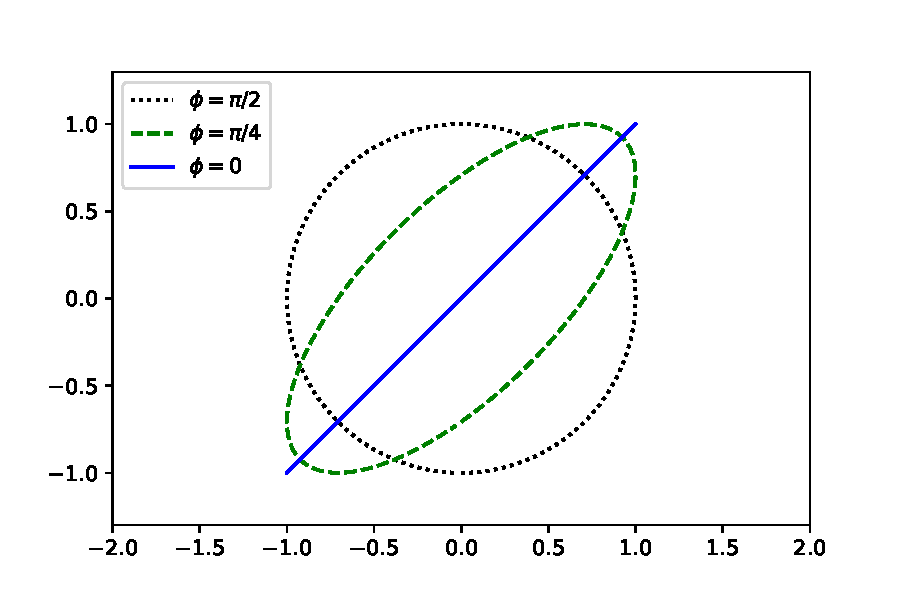
\includegraphics[width=0.50\textwidth]{figs/labs/filters/scope_xy.pdf}
\end{center}
\caption{\label{fig:scopexy} 
Expected scope traces in $XY$ display mode for a relative phase $\phi=\pi/2$, 
$\phi=\pi/4$, and $\phi=0$.  It is easy, accurate, and somehow deeply satisfying to tune the frequency until the ellipse collapses into itself, forming a line.}
\end{figure}

We'll measure the actual resonant frequency using a trick: an $XY$ mode of the scope.  
%During normal use, your oscilloscope displays the voltage of each channel versus
%time.  But there is an $XY$ mode available under the display options.
%In this mode, the scope displays the voltage of channel one versus the
%voltage of channel two.  
When in $XY$ mode, two out-of-phase signals
yield an ellipse.  But, as shown in Fig.~\ref{fig:scopexy} when both
channels are perfectly in phase, the ellipse collapses to make a
diagonal line. 
\begin{measurement} You can set you scope in XY mode and adjust the
frequency until the ellipse collapses to quickly and accurately find
the resonance frequency. Record the value in your logbook. Add comment in your logbook about how this measurement  compares to the calculated resonance frequency.
\end{measurement}
\begin{figure}[htbp]
\begin{center}
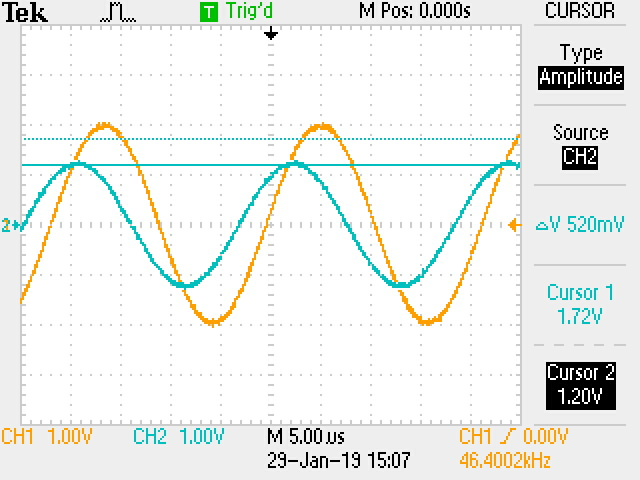
\includegraphics[width=0.45\textwidth]{figs/labs/filters/qscope.jpg}
\end{center}
\caption{\label{fig:qscope} Set Cursor 1 to the peak of Signal 2 at the resonant frequency, then set Cursor 2 to this value times $1/\sqrt{2}$.  The frequencies $f_+$ and $f_-$ can be determined by adjusting the frequency until the output amplitude reaches the level of Cursor 2, as shown here for $f_-$.
}
\end{figure}


\begin{measurement} One you determine the resonant frequency, switch back to the normal
display mode and determine the bandwidth.  The easiest way to obtain
this is to use the cursors to measure the peak voltage of your output
signal.  Multiply this by a factor of $1/\sqrt{2}$ to determine
the $-3~\rm dB$ amplitude and set the second cursor at this value, as
shown in Fig.~\ref{fig:qscope}.  Now adjust the frequency above and
below the resonant frequency and record at which frequencies the
amplitude reaches this line. Calculate the bandwidth and record it in your logbook.
\end{measurement}

\begin{measurement} From your measurement of $f_0$, $f_+$, and $f_-$ calculate the
measured $Q$-factor of your circuit. Record this value in your logbook. 
\end{measurement}


\noindent
This is a \textbf{sign-off point} for this lab. 

\section{Lissajous Figures Analysis}

\begin{plot} Reproduce fish pattern using scientific
python to draw the parameterized shape.  For
example, see Fig.~\ref{fig:pythonlissajous}. \end{plot}
\begin{plot} Reproduce  parabola pattern. \end{plot} 
\begin{plot} Reproduce crown pattern. \end{plot}

One way to approach this problem is to set the period to $1~\mu s$.
The functions should be evaluated at 1000 discrete times within the
interval from 0 to $1~\mu s$.
\begin{verbatim}
     t = np.linspace(0,1,num=1000)
\end{verbatim}
Define a fundamental angular frequency $\omega_0 = 2 \pi~\rm kHz$:
\begin{verbatim}
     w = 2*np.pi
\end{verbatim}
With these definitions, we would define:
\begin{verbatim}
     x = np.sin(4*w*t)
\end{verbatim}
to obtain $x$ points corresponding to $f=4~\rm kHz$ sine function.

When plotting your curves, use:
\begin{verbatim}
       plt.axis('equal')
\end{verbatim}
to keep the unit aspect ratio used by your scope.
%You can display your scope traces in python using the Image library like this:
%\begin{verbatim}
%       import Image
%
%       image = Image.open('myscope.jpg')
%       image.show()
%\end{verbatim}

\begin{figure}[htbp]
\begin{center}
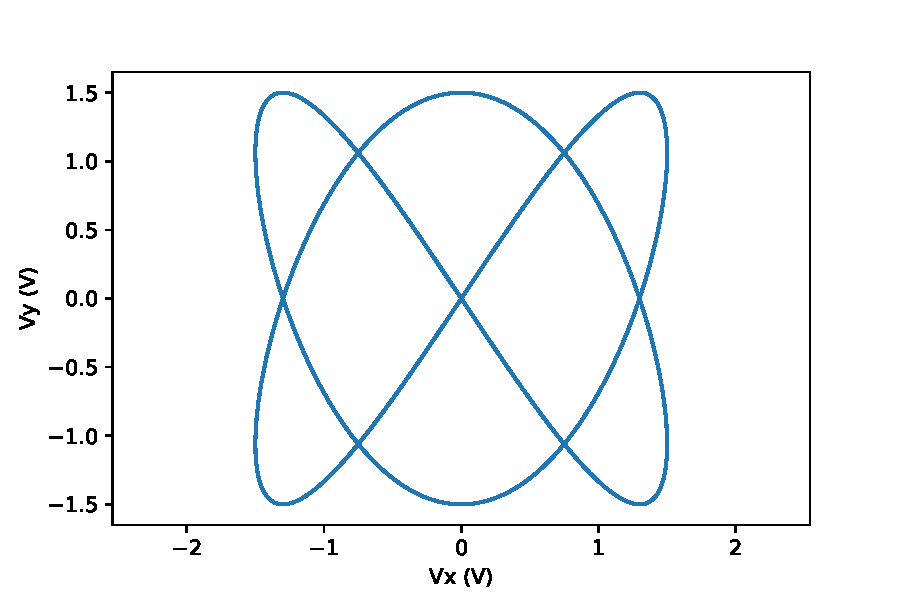
\includegraphics[width=0.45\textwidth]{figs/labs/lissajous/pythonlissajous.pdf} 
\caption{Lissajous curve constructed using Scientific Python corresponding to the scope trace in Fig.~\ref{fig:tracelissajous}a.}
\label{fig:pythonlissajous}
\end{center}
\end{figure}
